%!TEX program = xelatex
%!TEX TS-program = xelatex
%!TEX encoding = UTF-8 Unicode

% ================ 导言区 ================ 
% usepackage + global settings
% \documentclass[lang = cn, a4paper, 12pt]{article}  % report, book, proc, slides, minimal
% \usepackage[UTF8, scheme=plain]{ctex}  % CJK 和 xeCJK etc 的进一步封装
\documentclass[a4paper, 12pt]{ctexart}  % ctex + article
\usepackage[left = 1.25in, right = 1.25in, top = 1in, bottom = 1in]{geometry}
\usepackage{amsmath} % American Mathematical Society
\usepackage{amsfonts}
\usepackage{amsthm}
\usepackage[makeroom]{cancel}
\usepackage{graphicx}
\usepackage{float}

\title{\textbf{MATLAB in Economics and Management}}
\author{本科金融系 17020083 许楚楚} 
\date{\zhtoday}


% ================ 正文区================ 
\begin{document} 
\maketitle

\begin{abstract}本篇解决了老师布置的5道关于Matlab的题目,分别使用了栈,分枝定界法,最速下降法,Scaling方法和FIBONACCI search的方法,每一道题主要围绕着解题思路、代码实操、结果分析三个方面进行阐述。注:本报告用\LaTeX{}格式编写,源代码可以在压缩包中获得。
\end{abstract}
\tableofcontents

% ================ 第一题================ 
\section{Problem Set 1: 栈的使用}
\subsection{题目}
八皇后问题是一个以国际象棋为背景的问题:如何能够在8x8的国际象棋棋盘上放置八个皇后,使得任何一个皇后都无法直接吃掉其他皇后。为了达到此目的,任两个皇后都不能处于同一条横行、纵行或斜线上。

\textbf{要求:}使用数据结构中的栈实现,最终结果采用矩阵形式输出。

\subsection{解题思路}
 本题在求解过程中没有采用任何技巧,使用的是暴力枚举(brute force),利用递归的方法(recursion)实现深度优先的逐次枚举。为了从一定程度上降低复杂度(complexity),在遇到不合适的解的时候直接终止(break)后续棋子的摆放程序,跳至下一次尝试。
\subsection{代码实操}
首先定义了基本的变量,其中包含3个全局变量(global variable)依次为:\verb|condense_board|、\verb|solution|和\verb|n|。\verb|condense_board|是1x8的行向量,用于表示一整个棋盘,例如\verb|condense_board|中第5个元素值为8则表示第5行的皇后放在第8列。\verb|solution|是为了记录符合条件的八皇后问题解的变量,n表示的是棋盘的大小(在这里是8x8)。主要的程序操作还是由\verb|function search_at_depth(y1)|实现,其中输入参数y1是需要决定皇后摆放位置的行数。该函数实现的主要逻辑判断有:
\begin{enumerate}
\item 被检查行是否是第1至8行中的一行,如果是则为该行选择皇后位置--逐次在第\verb|y1|行的第1至8列尝试皇后的位置,如果皇后的列数位置与之前的皇后一样(\verb|x1 == x2|),尝试失败;如果皇后的斜对角存在其他皇后(\verb|(y1+x1) == (y2+x2)| 和\verb|(y1-x1) == (y2-x2)|),尝试也失败。上述采割条件都通过后,才算合格,进入下一行的测试。这里通过递归的方法实现\verb|search_at_depth(y1+1)|。
\item 如果输入行数大于8,说明该方案已经通过前面8轮测试,为可行解,则输出该解;
\item 如果上述条件皆不符合,i.e. 输入行数非大于1的整数,说明输入有问题,报错。
\end{enumerate}

\subsection{结果分析}
最终产生了92种可能的摆放情况,在此列举第34种\footnote{The writer's lucky number}:

\begin{verbatim}
The 34th solution
     0     0     0     1     0     0     0     0
     0     1     0     0     0     0     0     0
     0     0     0     0     0     0     1     0
     0     0     0     0     1     0     0     0
     1     0     0     0     0     0     0     0
     0     0     0     0     0     0     0     1
     0     0     0     0     0     1     0     0
     0     0     1     0     0     0     0     0
\end{verbatim}

% ================ 第二题================ 
\section{Problem Set 2: 最大化目标函数的分枝定界法}
\subsection{题目}
\begin{enumerate}
\item 初始求解整数规划的松弛问题:求解其松弛线性规划,若为整数解,极为整数规划的最优解。否则,初始下界设为$-\infty$。
\item 建立分枝树:在任何一个(子)问题中,从不满足整数要求的变量中选出一个进行处理,通过加入一对互斥的约束将一个(子)问题分支为两个受到进一步约束的子问题,缩小搜索的区域。由此,子问题若不满足整数要求,则进一步向下分枝,形成一个分枝树。
\item 定界与剪枝:通过不断分枝和求各个子问题,分枝定界法将不断修正已经得到的最优整数解确定的下界。其中,求解子问题可能出现以下结果:
	\begin{itemize}
	\item 无可行解,无须继续分枝
	\item 得到一个整数解,无需继续分枝,更新下界
	\item 得到一个非整数解,视目标函数值的情况决定剪枝还是继续分枝
	\end{itemize}
\item 按照上述步骤迭代,每当下界被修改以后,应当检查所有还没有求解过的子问题并剪去那些目标函数值小于新的下界的子问题。

\textbf{要求:}使用编写的程序求解一个需要迭代两次以上的整数规划问题。
\end{enumerate}

Example 2.16  用分枝定界法求解整数规划问题
\begin{equation*}
max \qquad x_{1}+x_{2}
\end{equation*}
\begin{equation*}
\text{s.t.} \qquad 
\begin{cases}
4x_{1}-2x_{2}\geq 1, \\
4x_{1}+x_{2}\leq 11,  \\
2x_{2}\geq 1,  \\
x_{1}, x_{2}\geq 0\text{且取整数值}.
\end{cases}
\end{equation*}

\subsection{程序设计思路}
本题旨在利用解决线性规划的方法解决整数规划,运用的是分枝定界法(branch-and-bound method)。首先需要标准化上述整数规划问题为Matlab的标准型,除去整数约束,得到松弛线性规划,该松弛线性规划问题标准化结果如下:
\begin{equation*} % obj
min \qquad -x_{1}-x_{2}
\end{equation*}
\begin{equation*} % constraint
\text{s.t.} \qquad 
\begin{cases}
-4x_{1}+2x_{2}\leq -1, \\
4x_{1}+x_{2}\leq 11,  \\
0x_{1}-2x_{2}\leq -1,  \\
x_{1}, x_{2}\geq 0.
\end{cases}
\end{equation*}

在Matlab中初始化问题代码如下,得到的解并非是整数解,因此我们需要建立分枝树,通过分枝定界法排查最优整数解。
\begin{verbatim}
c = [-1;-1];
A = [-4 2; 4 1; 0 -2];
b = [-1; 11; -1;];
lb = [0; 0];
up = [Inf; Inf];
\end{verbatim}

接下来就是代码实现的部分,主要的思路是,先求除去整数条件后的解松弛线性规划问题,并对解进行判定。如果无解,说明条件更为严格的整数规划问题也无解;如果返回整数解,即为整数规划问题的解;如果返回非整数解,进入分枝定界法的运行。分枝定界法的运行流程如下:输入主枝(mainNode)的参数求解线性规划问题,在进入分枝环节前需要做3次判定:1. 判定是否有解,无解则剪枝,\verb|return 0;|;2. 目标函数值是否低于当前上界(lowerBound),如果不低于当前上界,则没有继续运行的意义,剪枝;3. 解是否为整数解,如果是,更新当前上界(upperBound),存储决策变量和目标函数值至candidnate solution中(\verb|solution|),剪枝;如果解非整数解,则分枝。分枝部分需要做的就是通过改变上下界的取值收紧约束条件,利用recursion的原理在此调用函数branchbound得到2个分枝。

注:在传统分枝定界求解时,是对下界进行设定,而计算机的思维与人不同,需要将最大化问题转换为最小化问题,随之设定的应该是上界而非下界。

\subsection{结果分析}
通过运行主函数文件\verb|main.m|中的test case 2可以得到如下解。
\begin{verbatim}
===============================================

The optimal integer solution is:     2     3

The obj value is:    -5

===============================================
\end{verbatim}

该结果与\verb|doubleConfirm.m| 文件中通过Matlab内置命令intlinprog得到的结果一致。如果需进一步确认可以使用\verb|main.m|和\verb|doubleConfirm|给出的test case 1进行测试或者自定函数。


% ================ 第三题================ 
\section{Problem Set 3: 最速下降法}
\subsection{题目}
考虑下面的问题
\begin{equation}
\text{min} \qquad 5x^2+5y^2-xy-11x+11y+11
\end{equation}

找出满足一阶必要条件的解,证明该解为全局最优解。若用最速下降法求解该问题,收敛率是多少?选定$x=y=0$为初始点,最速下降法(最多)需要多少次迭代才能将函数值降至$10^{-11}$?

\subsection{找出满足一阶必要条件的解}
第一小问:根据一阶必要条件的的推论 \footnote{Corollary 2.1: Let $\Omega$ be a subset of $\mathbb{R}^n$  and let $f\in C^1$ be a function on $\Omega$. If $x^\ast$ is a relative minimum point of $f$ over $\Omega$ and if $x^\ast$ is an interior point of  $\Omega$, then $\bigtriangledown f(x^\ast)d = 0$.},可知满足条件的解出现在梯度为0的时候,则利用该条件在Matlab中进行实操。在Matlab中需要先输入定义符号目标函数,利用gradient命令得到目标函数关于x和y的偏导数,再利用solve命令得到当偏导数为0时的解。找到的满足一阶必要条件的解为$x=1, y=-1$,此时目标函数的值为0。

\subsection{证明该解为全局最优解}
第二小问:这里我们首先需要利用Theorem 2.3 \footnote{Theorem 2.3: Let $f\in C^2$. Then $f$ is convex over a convex set $\Omega$ containing an interior point if and only if the Hessian matrix F of $f$ is positive semidefinite.}“若目标函数的海赛矩阵是正定的,该函数就是凸函数”来证明目标函数为定义在凸集上的凸函数。再根据Theorem 2.4 \footnote{Theorem 2.4: Let f be a convex function defined on the convex set $\Omega$. Then the set $\Gamma$ where $f$ achieves its minimum is convex, and any relative minimum of $f$ is a global minimum}“凸函数的局部最优解就是全局最优解”证明在第一小问中得到的解是全局最优解。通过利用det命令求顺序主子式,求得得顺序主子式解大于0,说明目标函数为凸函数,那么第一问得到的局部最优解即全局最优解。

\subsection{求解最速下降法的收敛率}
首先利用eig命令求出海赛矩阵\textbf{H}的特征值,再用max和min命令求出特征值中最大和最小的特征值,得到r(condition number)等于最大特征值除以最小特征值,最后收敛率(covergence ratio)也由相应公式得到,为 0.0100。

\subsection{最多迭代次数}
\begin{proof}
根据Theorem 2.8\footnote{Theorem 2.8: For any $x_{0}\in \mathbb{R}^n$, the steepest descent method converges to the unique minimum point $x^*$ of f. Further more, there holds at every step k, $E(x_{k+1})\leq ( \frac{A-a}{A+a} ) ^2 E(x_{k})$ },收敛的最差情况是:\[E(x_{k+1}) = \bigg(\frac{A-a}{A+a}\bigg)^2 E(x_{k})\]

再根据$E(x_{k})$的定义\footnote{$E(x) = \frac{1}{2}(x-x^\ast)^t H (x-x^\ast)$}、初始条件$x_{0} = (0,0)$和收敛率$= 0.01$,得到:

\[E(x_{0}) =11\] 
\[E(x_{1}) =0.01E(x_{0}) = 0.11 \]
\[E(x_{2}) =0.01E(x_{1}) = 0.0011 \]
\[\cdots \qquad \cdots \]

设经过$n$次的迭代后$E(x_{k})\leq 10^{-11}$
 \[11*0.01^n=10^{-11} \]
 \[n = log_{0.01}(10^{-11}) \]
 \[n=6.0207\]
\end{proof}

所以得出结论:最多只需要经过7次的迭代就可以将函数值降至$10^{-11}$。虽然说理论上,最多迭代的次数不会超过7次,但是通过运行文件\verb|gradient.m|中question 4的部分,得到count = 1, 即在实际操作中仅需进行一次迭代便可得出最优解。


% ================ 第四题================ 
\section{Problem Set 4: Scaling方法}
\subsection{题目}
已知目标函数
\begin{equation}
f(x,y)=x^2+5xy+y^4-25x-8y
\end{equation}
用最速下降法求最小值。
现采用scaling方法,其原理是令Hessian矩阵主对角线上元素的值近似相等。令$z=7y$对上式做代换,重新用最速下降法求最小值,并比较两次迭代次数的结果。
\subsection{可视化}
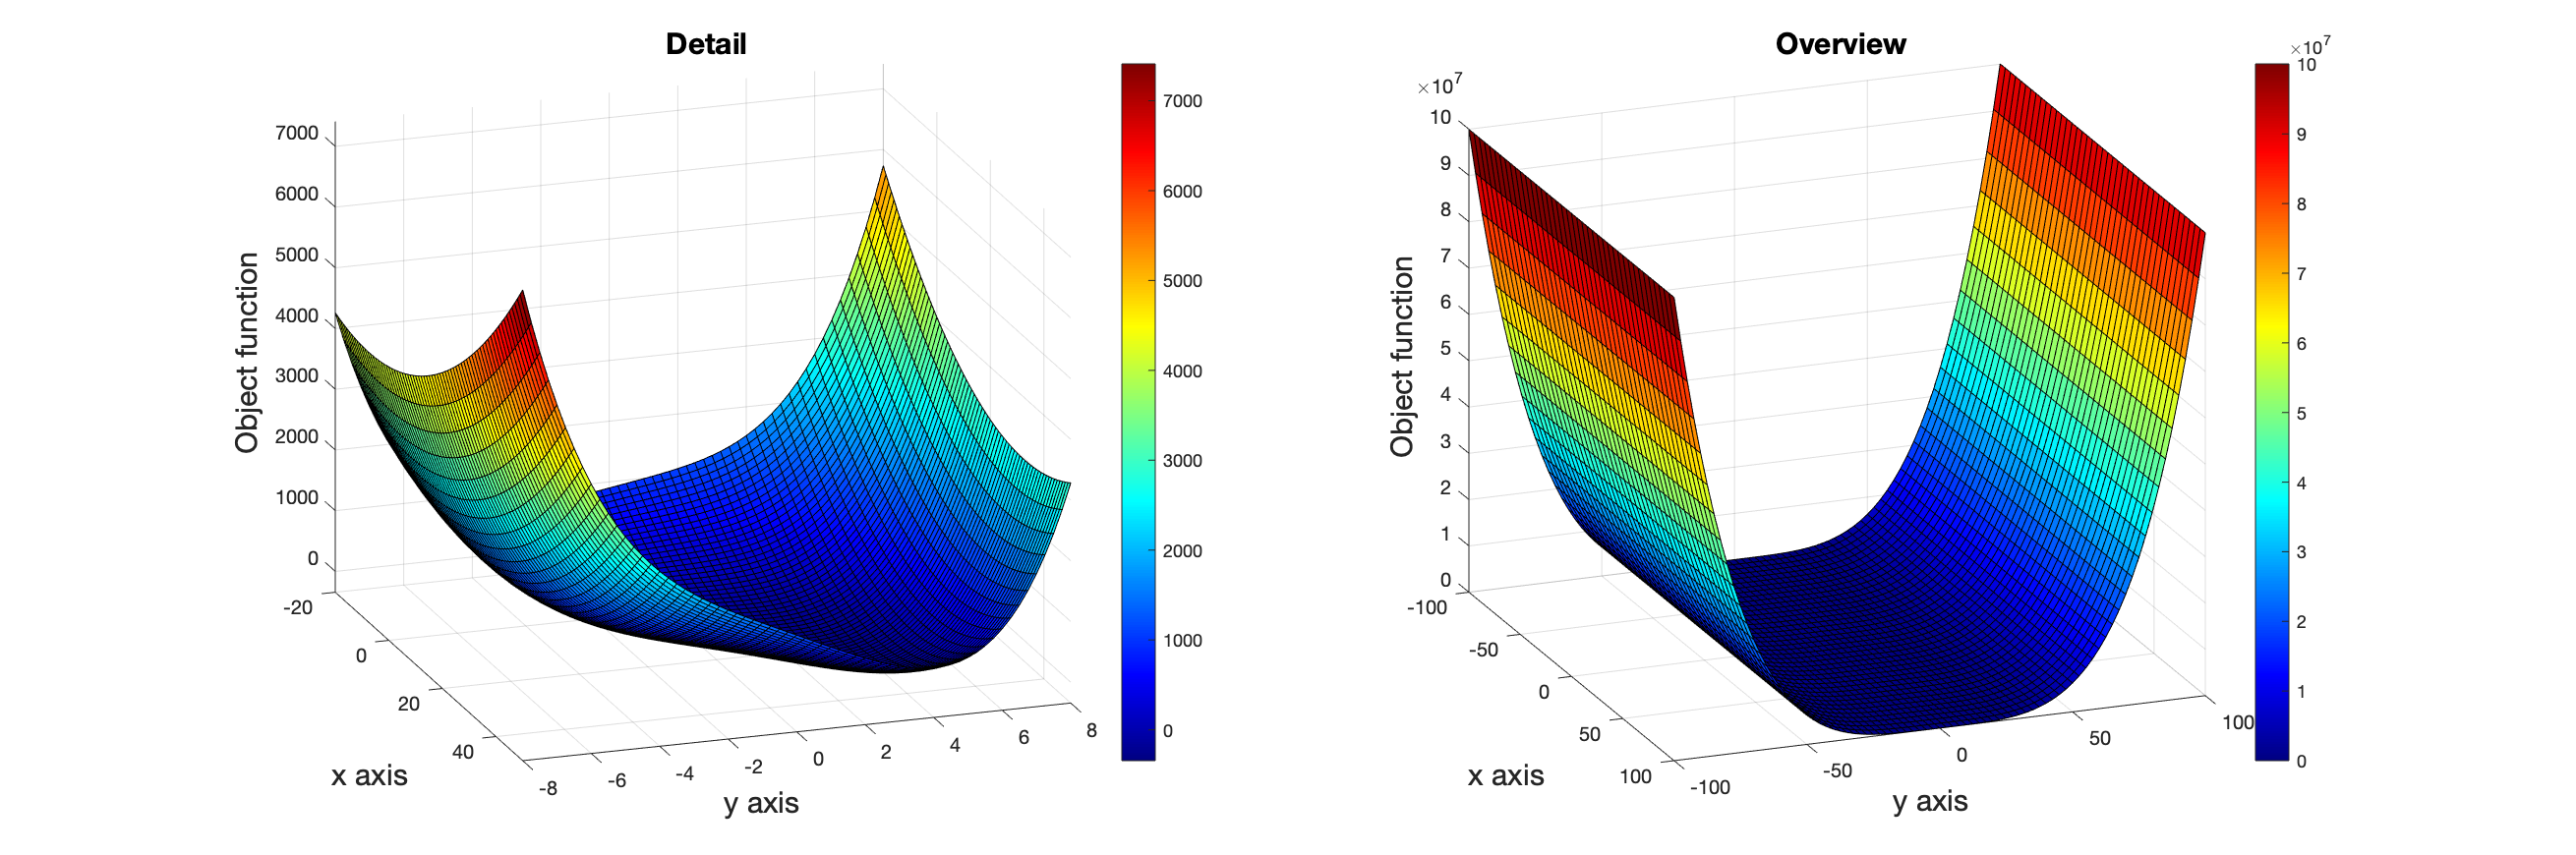
\includegraphics[height=2in, width=6in]{visualization.png}

该函数底部看似是对称平滑的曲面(右图),但实际上底部是凹凸不行、不对称的(左图)。
\subsection{程序设计思路}
首先利用\verb|fminsearch|函数计算出目标函数的最小值,得出当$x=20, y = 3$的时候,目标函数值最小,为-340。接下来是进行最速下降的操作:定义符号变量x, y, z, a\footnote{a为最优步长},利用\verb|gradient|命令计算出梯度表达式,开始迭代操作。这里利用\verb|while|循环设定迭代结果与实际最小值之间的误差必须小于0.000001才算迭代得到最优解。在\verb|while|循环内主要做2件事情:一、确定方向;二、确定最优步长。方向是梯度$\bigtriangledown f(x_{k})$取反方向,最优步长$\alpha$是通过对$f(x_{k}-\alpha \bigtriangledown f(x_{k})^t)$求导、设定求导后函数为0得到,在Matlab中的具体实现是:\verb|double(solve(diff(fa,a),'Real',true))|,因为可能会出现复数解,因此需要在\verb|solve|中设定参数\verb|Real|确保得到整数解,\verb|double|是为了将分数解转换为小数存储(如果以分式形式存储,运行会非常慢,这里是对于精确度和运行速度做了一个tradeoff)。以此迭代循环,直至和最优值之间的误差小于0.000001结束循环。

上述是对原函数的操作,对于缩放(Scaling)后的目标函数,操作方法实际上是完全一致的,只是需要在个别函数名称上进行改变。
\subsection{结果分析}
通过运行beforeScaling.m文件,得到结果如下,第一个数字是x的取值、第二个数字是y的取值、第三个数字是最终目标函数的取值。为了得到误差小于0.000001的解,一共进行了79次尝试、78次迭代。
\begin{verbatim}
The 79 time try
Solution: 
   19.9990
    2.9999

Object value: -343.0000
Condition number:  61.3327
\end{verbatim}

接下来让我们看一下在Scaling之后的程序运行效率。通过运行afterScaling.m文件,得到结果如下,不同于Scaling之前,第二个数字是z的取值,大约为beforeScaling.m运行得到y值的3倍,符合预期。由此可见,为了得到误差小于0.000001的解,仅仅只进行了12次尝试、11次迭代,运行效率大大提高。
\begin{verbatim}
The 12 time try
Solution: 
   19.9998
   20.9995

Object value: -343.0000
Condition number:   2.0453
\end{verbatim}

差距的原因是因为scaling前后的海赛矩阵不同,导致了对应特征矩阵的最大和最小的特征值不一样,得到的$r$(condition number)不一样,收敛率也不同。通过在源代码中加入计算$r$的代码,让计算机输出了scaling前后的$r$,scaling前的$r$大约在61左右,而scaling后的$r$降至到了2左右,根据Theorem 2.8 \footnote{Theorem 2.8: For any $x_{0}\in \mathbb{R}^n$, the steepest descent method converges to the unique minimum point $x^*$ of f. Further more, there holds at every step k, $E(x_{k+1})\leq ( \frac{A-a}{A+a} ) ^2 E(x_{k})$ }, $( \frac{A-a}{A+a} ) ^2 = (\frac{r-1}{r+1})^2, $ $r$越小说明收敛的速度越快,由此可以说明缩放后收敛速度更快的原因。
% ================ 第五题================ 
\section{Problem Set 5: FIBONACCI搜索}
\subsection{题目}
对于FIBONACCI搜索方法,令搜索区间的初始长度为$d_{1}=c_{2}-c_{1}$
\begin{enumerate}
\item 证明$d_{k}=\frac{F_{N-k+1}}{F_{N}}d_{1}$
\item 插入两个试验点后计算函数值,若第一次迭代的结果是保留左端点$c_{1}$,求下一个插入点坐标的两种表达式,并验证它们的等价性。
\end{enumerate}

\subsection{$d_{k}$与$d_{1}$关系证明}
\begin{proof}
假设 $d_{i}$  是进行$i$次操作后不确定区间的宽度,N是总的操作次数

根据前一项与后一项之间的比为fibonacci数列之比,得:
\[ d_{2}  =  \bigg(\frac{F_{N-1}}{F_{N}}\bigg)d_{1} \]
\[ d_{3}  =   \bigg(\frac{F_{N-2}}{F_{N-1}}\bigg)d_{2} \]
\[  \cdots \]
\[ d_{k-1}  =   \bigg(\frac{F_{N-k+2}}{F_{N-k+3}}\bigg)d_{k-2} \]
\[ d_{k}  =   \bigg(\frac{F_{N-k+1}}{F_{N-k+2}}\bigg)d_{k-1} \]
根据迭代法消元得:
\[ d_{k} =  \bigg(\frac{F_{N-k+1}}{\cancel{F_{N-k+2}}}\bigg) \cdot \bigg(\frac{\cancel{F_{N-k+2}}}{\cancel{F_{N-k+3}}}\bigg) \cdot \dots  \cdot \bigg(\frac{\cancel{F_{N-2}}}{\cancel{F_{N-1}}}\bigg) \cdot \bigg(\frac{\cancel{F_{N-1}}}{F_{N}}\bigg) d_{1} \]
\[ d_{k}=\frac{F_{N-k+1}}{F_{N}}d_{1} \]
\end{proof}

\subsection{插入表达式等价性证明}
方法一是通过更新后上下界$b_{k}$和$a_{k}$与中间插入点$t_{1}$和$t_{2}$的关系而得。在当前题目给定条件下,第一次迭代结果是保留左点点$c_{1}$,那么新的下界是原来的$a_{0}$、新的上界是原来的$t_{2}$、新的的$t_{2}$是原来的$t_{1}$,那么我们现在需要求解的便是新的$t_{1}$值。假定新的$t_{1}$为$t_{1}'$,根据$t_{1}'$距离上界的距离为区间长$d2$乘以当前fibnacci序列比例,得到表达式 1: \begin{equation} t_{1}' = b_{1} - \bigg( \frac{F_{k-2}}{F_{k-1}}  \bigg) d_{2}  \end{equation}

方法二是根据画图得到了表达式 2: 
\begin{equation}
t_{1}' = a_{0} + d_{2} - d_{3}
\end{equation}
\begin{figure}[h]
\centering
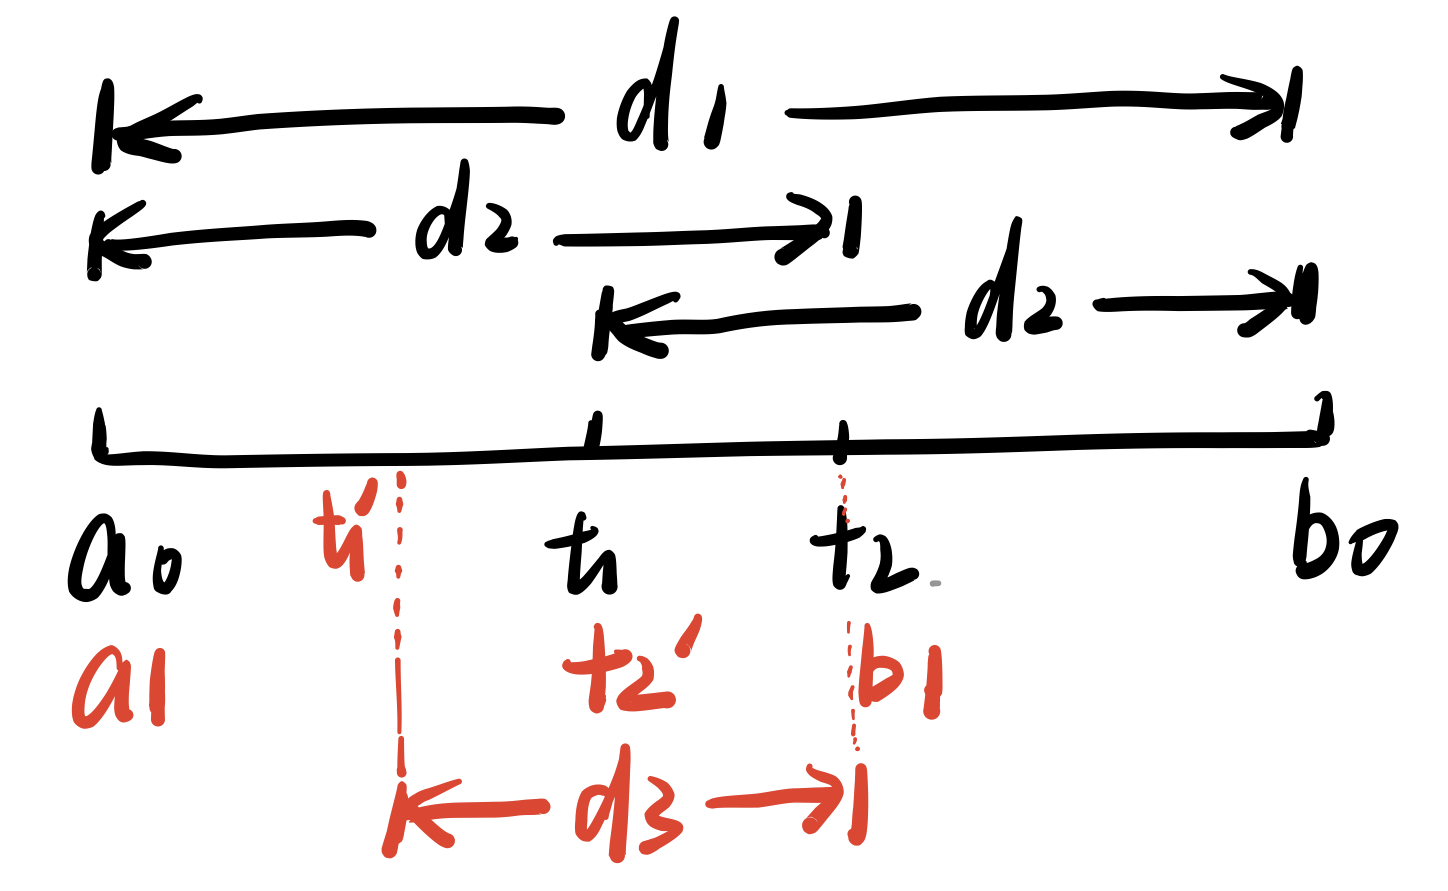
\includegraphics[height=1.75in, width=3in]{fibnacci.jpg}
\caption{表达式2图例}
\end{figure}

\begin{proof}
通过等式变换关系,表达式 1 可以通过下述转变得到:
\begin{align*}
t_{1}' &= b_{1} - \bigg( \frac{F_{k-2}}{F_{k-1}}  \bigg) d_{2} 	\\
t_{1}' &= b_{1} - d_{3}
\end{align*}

通过等式变换关系,表达式 2 可以通过下述转变得到:
\begin{align*}
t_{1}' &= a_{0} + d_{2} - d_{3} \\
t_{1}' &= t_{2} - d_{3} \\
t_{1}' &= b_{1} - d_{3} 
\end{align*}

两者等价性得证。
\end{proof}
\end{document} 




% ================ cheat sheet ================ 
% 1. 特殊字符
% \#  \$  \%  \{  \}  \_
% \^{}  \~{}
% \textbackslash

% 2. 标点符号(en)
% 单引号'    
% 双引号'+'
% 连字号- 
% 短破折号-- 
% 长破折号---
% 省略号 \ldots, \dots

% 3. 特殊西文符号与重音(参考教程)

% 4. 其他符号
% \P{} \S{} \dag{} \ddag{}
% \copyright{}
% \pounds{}
% \textasteriskcentered
% \textperiodcentered
% \textbullet
% \textregistered{}
% \texttrademark

% 5. format
% underline: \usepackage{ulem}  
% An example of \uline{some long and underlined words.}
% emphasize: \emph{emphasis}

% 6. newline
% \\ 
% \newline
% \nolinebreak

% 7. newpage
% \newpage
% \clearpage
% \nopagebreak

% 3.1.2 目录
% \tableofcontents  需要2次编译源代码
% \addcontentsline{toc}{<level>}{<title>}

% 3.3 交叉引用

% 3.4 脚注
% \footnote{<footnote>}

% 3.5.1 列表(详细参考书目)
% \begin{enumerate}
% \item...
% \end{enumerate}

% 3.5.5 代码环境
% 成段代码
% \begin{verbatim}
% \end{verbatim}
% 简单代码
% \verb|\LaTeX|

% 3.6 表格

% 3.7 图片
% \includegraphics[<option>]{<filename>}

% 3.8 盒子

% 3.9 浮动体

% 4.2 公式排版基础
% $$
% \begin{equation}
% \end{equation}
% 引用
% \label{Taylor's Expansion}
% \eqref{Taylor's Expansion}

% 4.2.1 数学模式
% 空格全部被忽略
% \quad \qquad
% 换行 \\
% \text{}
% \textbf{}

% 4.3.1. 数学符号
% \infty
% \dots
% \cdots
% \vdots for matrix
% \hdots for matrix

% 4.3.4 关系符
% \ne
% \ge
% \le
% \approx
% \equiv
% \propto
% \sim

% 4.3.5算符
% \nabla
% \partial

% 5.1.1 字体(refer to the handbook)
% \textrm{} roman
% \textsf{} sans serif
% \texttt{}  typewriter
% \textmd{}
% \textbf{}
% \textit{}
% \emph{}
% \textup{}

















